\experiment{System Calls}{04/10/2023}

\section*{Aim}
To familiarize the System calls such as fork, exec, getpid, exit, wait, close, stat,
opendir, readdir


\section{fork()}
\subsection{Description}
fork is used to create a new process
\subsection{Program}
\begin{lstlisting}[label={list:c_program:fork}]
#include<stdio.h>
#include<stdlib.h>
#include<unistd.h>
#include<sys/types.h>
int main(int argc, char **argv)
{
pid_t pid;
pid = fork();
if(pid==0)
{
    printf("It is the child process and pid is %d\n");
    exit(0);
}
else if(pid > 0)
{
    printf("It is the parent process and pid is %d\n");
}
else
{
    printf("Error while forking\n");
    exit(EXIT_FAILURE);
}
return 0;
}
\end{lstlisting}

\subsection{Output}
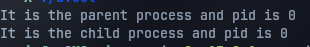
\includegraphics[]{Cycle_1/Outputs/fork.png}

\section{exec()}
\subsection{Description}
exec is used to replace the process’s memory space with a new program.
The exec system call is used to execute a file which is residing in an active process
\subsection{Program - exec.c}
\begin{lstlisting}[label={list:c_program:exec}]
#include <stdio.h>
#include <unistd.h>
#include <stdlib.h>
int main()
{
    char *args[]={"./another",NULL};
    execvp(args[0],args);
    printf("End\n");
}
\end{lstlisting}
\subsection{Program - another.c}
\begin{lstlisting}[label={list:c_program:exec2}]
int main()
{
    printf("This is another process\n");
    return 0;
}
\end{lstlisting}
\subsection{Output}
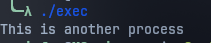
\includegraphics[]{Cycle_1//Outputs/exec.png}

\section{getpid()}
\subsection{Description}
getpid() is used to get the process ID of the process that calls that function
\subsection{Program}
\begin{lstlisting}[label={list:c_program:fork}]
#include <stdio.h>
#include <unistd.h>
int main()
{
int pid;
pid = fork();
if (pid == 0)
{
    printf("Process id : %d \n",getpid());  
}
return 0;
}
\end{lstlisting}

\subsection{Output}

\includegraphics[]{Cycle_1//Outputs/getpid.png}

\section{exit()}
\subsection{Description}
exit() is is used to terminate a process
\subsection{Program}
\begin{lstlisting}[label={list:c_program:exit}]
#include <stdio.h>
#include <stdlib.h>
#include<unistd.h>
#include <sys/types.h>

int main () {
  printf("Start of the program....\n");
  fork();
  printf("Exiting the program....\n");
  exit(0);
  printf("End of the program....\n");
  return(0);
}

\end{lstlisting}

\subsection{Output}
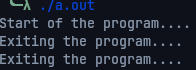
\includegraphics[]{Cycle_1//Outputs/exit.png}

\section{wait()}
\subsection{Description}
wait parent process can wait for a child process to terminate using wait system
call
\subsection{Program}
\begin{lstlisting}[label={list:c_program:exit}]
#include<stdio.h>
#include<unistd.h>
#include<stdlib.h>
#include<sys/wait.h>
int main()
{
  int pid=fork(); //creating child
  if(pid<0)
  {
    printf("fork failed!\n");
  }
  else if(pid==0)
  {
    printf("\nchild process %d executing\n",getpid());
    printf("calling program prg.c from child using exec\n");
    char* argv[]={"prg",NULL};
    execv("./prg",argv);
  }
  else
  {
    printf("parent process %d executing\n",getpid());
    int status;
    printf("parent waiting for child to terminate\n");
    int pid=wait(&status);
    printf("child process %d exited-parent wait over\n",pid);
    printf("parent process %d exits\n",getpid());
  }
}

\end{lstlisting}

\subsection{Output}
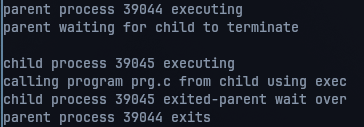
\includegraphics[]{Cycle_1//Outputs/wait.png}


\section{close()}
\subsection{Description}
close() is a system call used to close a file descriptor
\subsection{Program}
\begin{lstlisting}[label={list:c_program:exit}]
#include <stdlib.h>
#include <fcntl.h>
#include<unistd.h>
#include<stdio.h>

int main()
{
  size_t filedesc = open("testfile.txt", O_WRONLY | O_CREAT);
  if(filedesc < 0)
  {
    printf("Outside close\n");
    return 1;
  }
  if(close(filedesc) < 0)
  {
    printf("Inside close\n");
    return 1;
  }
  else
  {
    printf("File present\n");
  }
  return 0;
}
\end{lstlisting}

\subsection{Output}
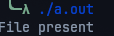
\includegraphics[width=0.5\linewidth]{Cycle_1//Outputs/close.png}

\section{stat()}
\subsection{Description}
Stat system call is a system call in Linux to check the status of a file such as to
check when the file was accessed
\subsection{Program}
\begin{lstlisting}[label={list:c_program:exit}]
#include <sys/types.h>
#include <sys/stat.h>
#include <stdio.h>
#include <time.h>

int main() {
  struct stat info;
  if (stat("/", &info) != 0)
    perror("stat() error");
  else {
    puts("stat() returned the following information about root f/s:");
    printf(" inode: %d\n", (int) info.st_ino);
    printf(" dev id: %d\n", (int) info.st_dev);
    printf(" mode: %08x\n", info.st_mode);
    printf(" links: %ld\n", info.st_nlink);
    printf(" uid: %d\n", (int) info.st_uid);
    printf(" gid: %d\n", (int) info.st_gid);
  }
  return 0;
}
\end{lstlisting}

\subsection{Output}
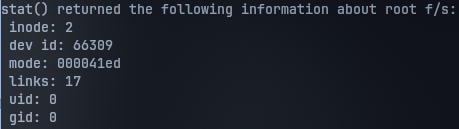
\includegraphics[]{Cycle_1//Outputs/stat.png}

\section{opendir() and readdir()}
\subsection{Description}
opendir() opens a directory stream corresponding to the directory name, and
returns a pointer to the directory stream. readdir() is used to read into a
directory.The function returns a pointer to a dirent structure.
\subsection{Program}
\begin{lstlisting}[label={list:c_program:exit}]
#include <stdio.h>
#include <dirent.h>

int main()
{
  DIR *folder;
  struct dirent *entry;
  int files = 0;
  folder = opendir("testdir");
  if(folder == NULL)
  {
    perror("Unable to read directory");
    return(1);
  }
  while( (entry=readdir(folder)) )
  {
    files++;
    printf("File %3d: %s\n",files,entry->d_name);
  }
  closedir(folder);
  return(0);
}
\end{lstlisting}

\subsection{Output}
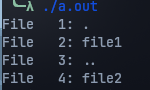
\includegraphics[width=0.5\linewidth]{Cycle_1//Outputs/opendir.png}


\section*{Result}
Implemented programs to demonstrate the use of fork, exec, getpid, exit, wait,
close, stat, opendir and readdir system calls